
%--------------------------------------------%
% Packages arranged by : Tsz Timmy Chan	     %
%                 Date : November 26th, 2016%
%--------------------------------------------%

\documentclass{TC}
\usepackage{TCcommon}

\title{TITLE HERE}	% Work Title Here.
\author{Tsz Timmy Chan}	% YOUR NAME HERE 

\usepackage[notes]{TCheader}
\usepackage{TCexamtitle}
%\renewcommand{\benediction}{" " - }
%\renewcommand{\quoteoftheday}{" " \\ - }
\begin{document}
Given some cone $D_i$ we can generate a cone $D_{i+1}$ such that $D_{i+1} \subset D_i$ by taking the Hilbert basis of $D$ (the original outer cone), and removing one extremal vector from this list. We then take the conical hull of the remaining vectors, giving us a $D_{i+1} \subset D$, where the lattice elements of $D_{i}$ by construction is exactly $\Hilb(D_{i+1}) + v$ for some $v$ not in $D_{i+1}$. This can be applied in such a way where given any arbitrary full dimensional lattice cone $C \subset D$.

\begin{lemma} \label{topdownposetlemma}
The Top Down algorithm generates cones $D = D_0 \supset D_1 \supset D_2 \supset \cdots$ such that each pair $D_{n+1} \subset D_{n}$ satisfy the poset condition \textbf{\ref{ConePosetCondition}}. 
\end{lemma}

As an application, these two types of extensions give us:

\begin{lemma}
$\mathrm{Cones}(d)$ has neither maximal nor minimal elements, other than the minimal element 0.
\end{lemma}
\begin{proof}
Given some cone $C \in \Cones(d)$, apply a Hilbert descend to find a cone that is lower on a poset, and apply a height-1 extension to obtain a cone higher on a poset chain.
\end{proof}

What does it mean that we do not know whether 0 is the smallest element? This means that while we know the 0 cone is contained in all other cones, we do not know if given any $C \supset 0$ we can find a finite sequence of cones so that $0 < C$ based on \textbf{\ref{ConePosetCondition}}.

A question was asked by Gubeladze and Micha\l{}ek in \cite{GubeladzePosetCones} on the elementary extensions: "Do either height 1 extensions or Hilbert basis descends generate the same poset $\mathrm{Cones}(d)$?" 

This above question is considered in five different ways in this paper, and in particular we focus on questions (3) and (4):
{
\begin{figure}[h]
\centering
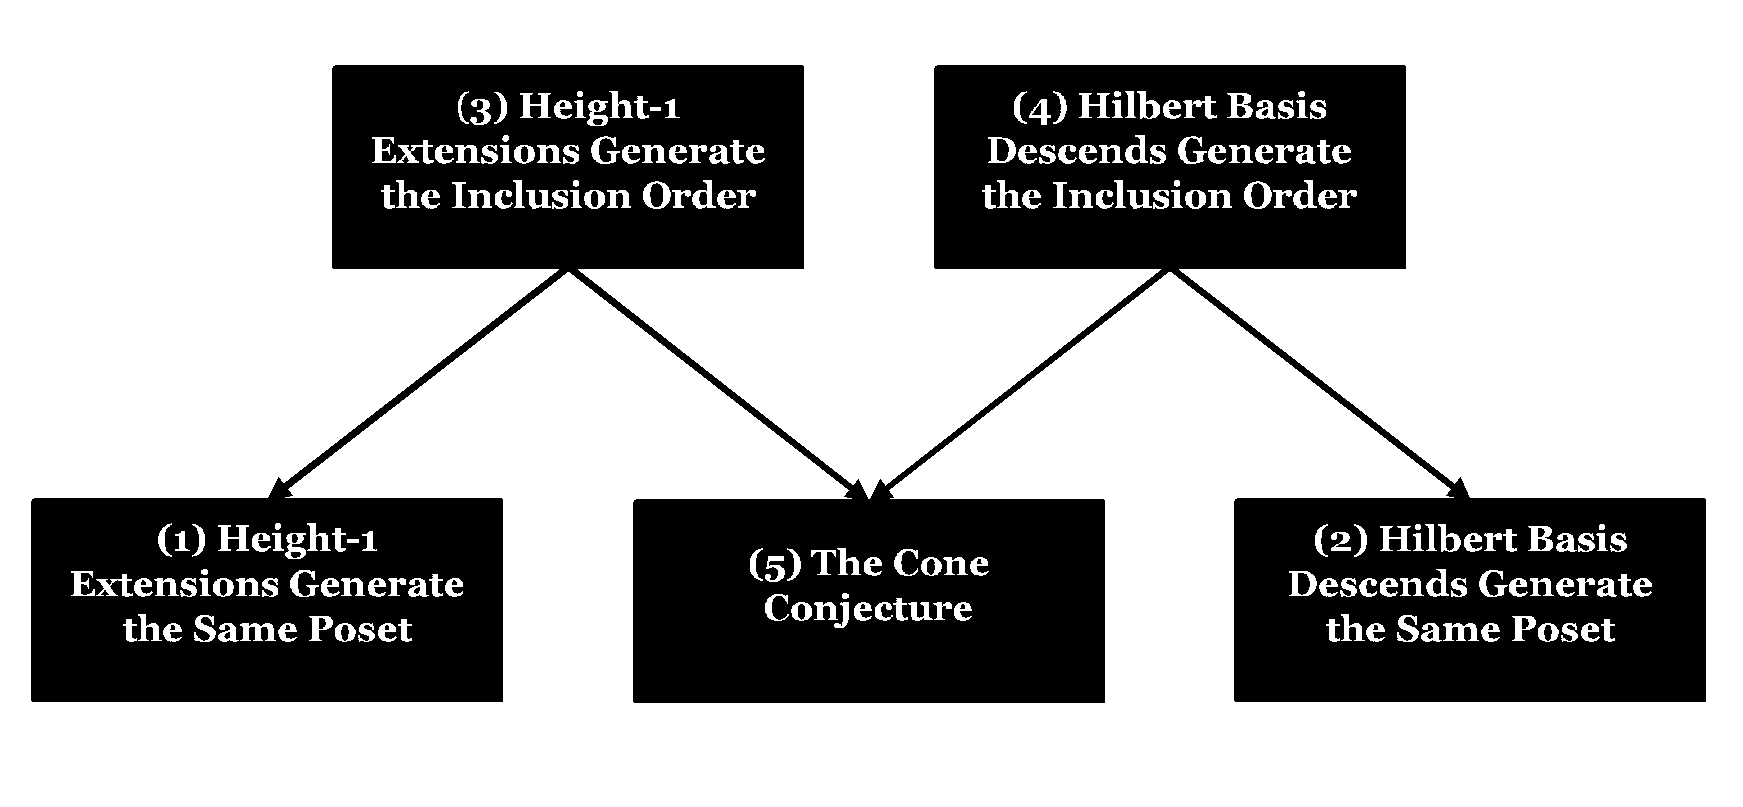
\includegraphics[width=.95\textwidth]{Questions}
\label{coneconjecturequestions}
\caption{Logical implications of the questions.}
\end{figure}
}
\begin{enumerate}[(1)]
\item Do Height-1 extensions generate $\Cones(d)$? This is a separate statement from the cone conjecture, since not all elementary extensions are of the form of Height-1 extensions.
\item Do Hilbert descends generate $\Cones(d)$? 
\item Do Height-1 extensions generate inclusion order? This is a stronger statement than the cone conjecture and would imply (1) if true. If this is true, then for any $C \subset D$ one can generate a finite chain $C = C_0 < C_1 <\ldots< C_n = D$ using height 1 extensions.
\item Do Hilbert descends generate the inclusion order?
\item The cone conjecture.

\end{enumerate}

The positive answer towards questions (3) and (4) above implies the cone conjecture, because they are both logically stronger statements. Furthermore, they imply questions (1) and (2) as well, respectively. 

The proof given in dimension 3 shows that the answer to question 5 is true in \cite{GubeladzePosetCones}; but it does not show 1 - 4. Our work provides statistical evidence in dimension 4 and 5 suggesting that the answer to questions 3~and~4 is no.


\end{document}